\footnotesize
\frame{\section{Introduzione}
\subsection[Problema]{Problema: segmentazione}
\frametitle{Problema}

\begin{block}{Analisi automatica ed in linea della deambulazione umana}
\begin{itemize}
	\item \textbf{analisi}: estrazione di parametri temporali della deambulazione (\textbf{Segmentazione})
	\item \textbf{automatica}: che funziona senza interventi umani
	\item \textbf{in linea }(\textit{online}): vincolo temporale sulla latenza tra verificarsi di un evento ed il tempo di rilevamento del sistema
\end{itemize}
\begin{columns}
\column{.3\textwidth} \hspace{0.5cm}
%\includegraphics[width=0.7\textwidth]{billeder/circuit} 
\column{.7\textwidth}
\end{columns}
\end{block}
}

%%%%%%%%%%%%%%%%%%%%%%%%%%%%%%%%%%%%%%%%%%%%%%%%%%%%%%%%%%%%%%%%%%%%%%%%%%%%%%%%%%%%%%%%%%%%%%%%%%%%%%%%%%%%%%%%%%%%%%%%%

\frame{\subsection[Soluzione]{Soluzione: Hidden Markov Models (HMM)}
\frametitle{Soluzione: prototipo}

\begin{block}{Logica}
\begin{itemize}
	\item \textbf{Modello stocastico per sequenze temporali della deambulazione}: HMM addestrata su $n$ soggetti 
	\item \textbf{Algoritmo di decodifica in linea}: versione in linea dell'algoritmo di Viterbi  
\end{itemize}
\end{block}

\begin{block}{Hardware}
\begin{columns}
	\column{.6\textwidth}
		\begin{itemize}
			\item \textbf{Acquisizione dati deambulazione}: giroscopio monoassiale contenuto in una \textbf{IMU} (Inertial Measurement Unit) 
			\item \textbf{Posizionamento}: collo del piede ed orientato con l'asse sensibile sul piano mediale-laterale
			\item \textbf{Trasmissione}: comunica dati e riceve comandi via \textit{Bluetooth}
		\end{itemize}
	\column{.35\textwidth}
		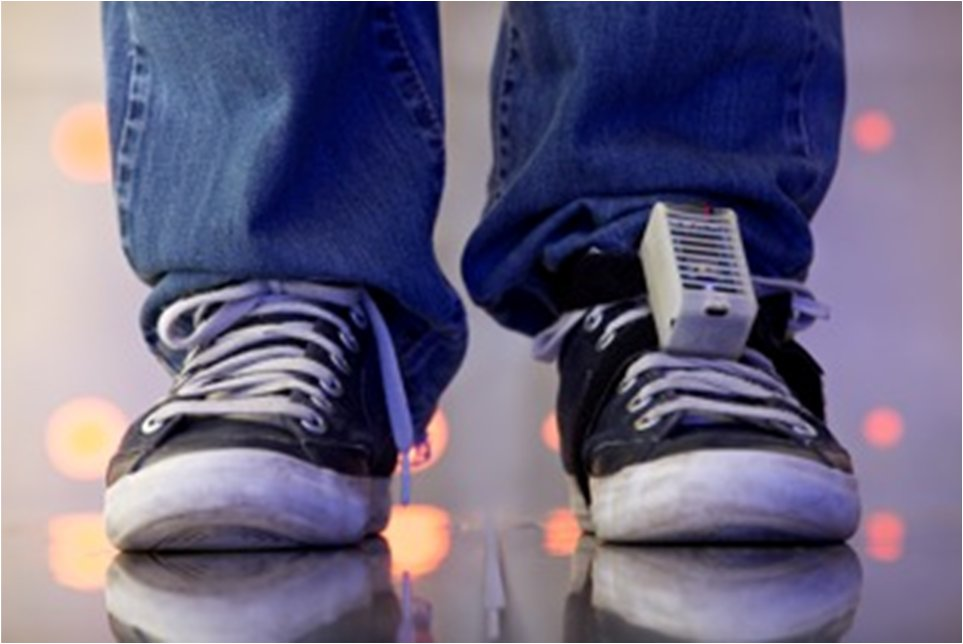
\includegraphics[width=.9\textwidth]{imgs/sensore.jpg}
	\end{columns}
\end{block}

\begin{block}{Software}
\begin{itemize}
	\item \textbf{Controllo, elaborazione e visualizzazione}: \textit{Smartphone} Android\tm
\end{itemize}
\end{block}
}

%%%%%%%%%%%%%%%%%%%%%%%%%%%%%%%%%%%%%%%%%%%%%%%%%%%%%%%%%%%%%%%%%%%%%%%%%%%%%%%%%%%%%%%%%%%%%%%%%%%%%%%%%%%%%%%%%%%%%%%%%
\frame{\subsection{Valutazione}
\frametitle{Valutazione del prototipo}

\begin{block}{Metodo di verifica del funzionamento}
\begin{itemize}
	\item Stima velocit� sistema ideato : $IMUspeed$
	\item Stima velocit� GPS: $GPSspeed$
	\item Confronto: $IMUspeed \approx GPSspeed$ ?
\end{itemize} 
\end{block}


}
